%!TEX root = ../document.tex
\chapter{Project Communication Management}

\section{Project decision process}

The decision making and reporting processes described below are related to daily challenges and decisions. Some challenges may result in project scope, resources or time. The change of the table needs to be handled by the change control process described in the change management. 

For decisions that do not have a significant impact on the scope, resources or timelines of the project, the project team has the discretion to decide. Decision making the first level escalation leader is the flying car project manager. The second-level reporting leader is the project director. Before reporting to a higher level, at a certain the level leadership office may not report more than twice. Need to get input from the steering committee or need to get most of internal consent decisions are limited to the following: (I) Decisions that have a significant impact on flying car project's existing business processes; (II) Decisions will affect flying car project key Policy decisions; (III) decisions that bring significant changes to the scope, timelines, functionality, or costs of the project. These are referred to as “significant Decision”. A decision flow chart is given on the next page, which details the process. 

\begin{figure}[!htb]
\centering
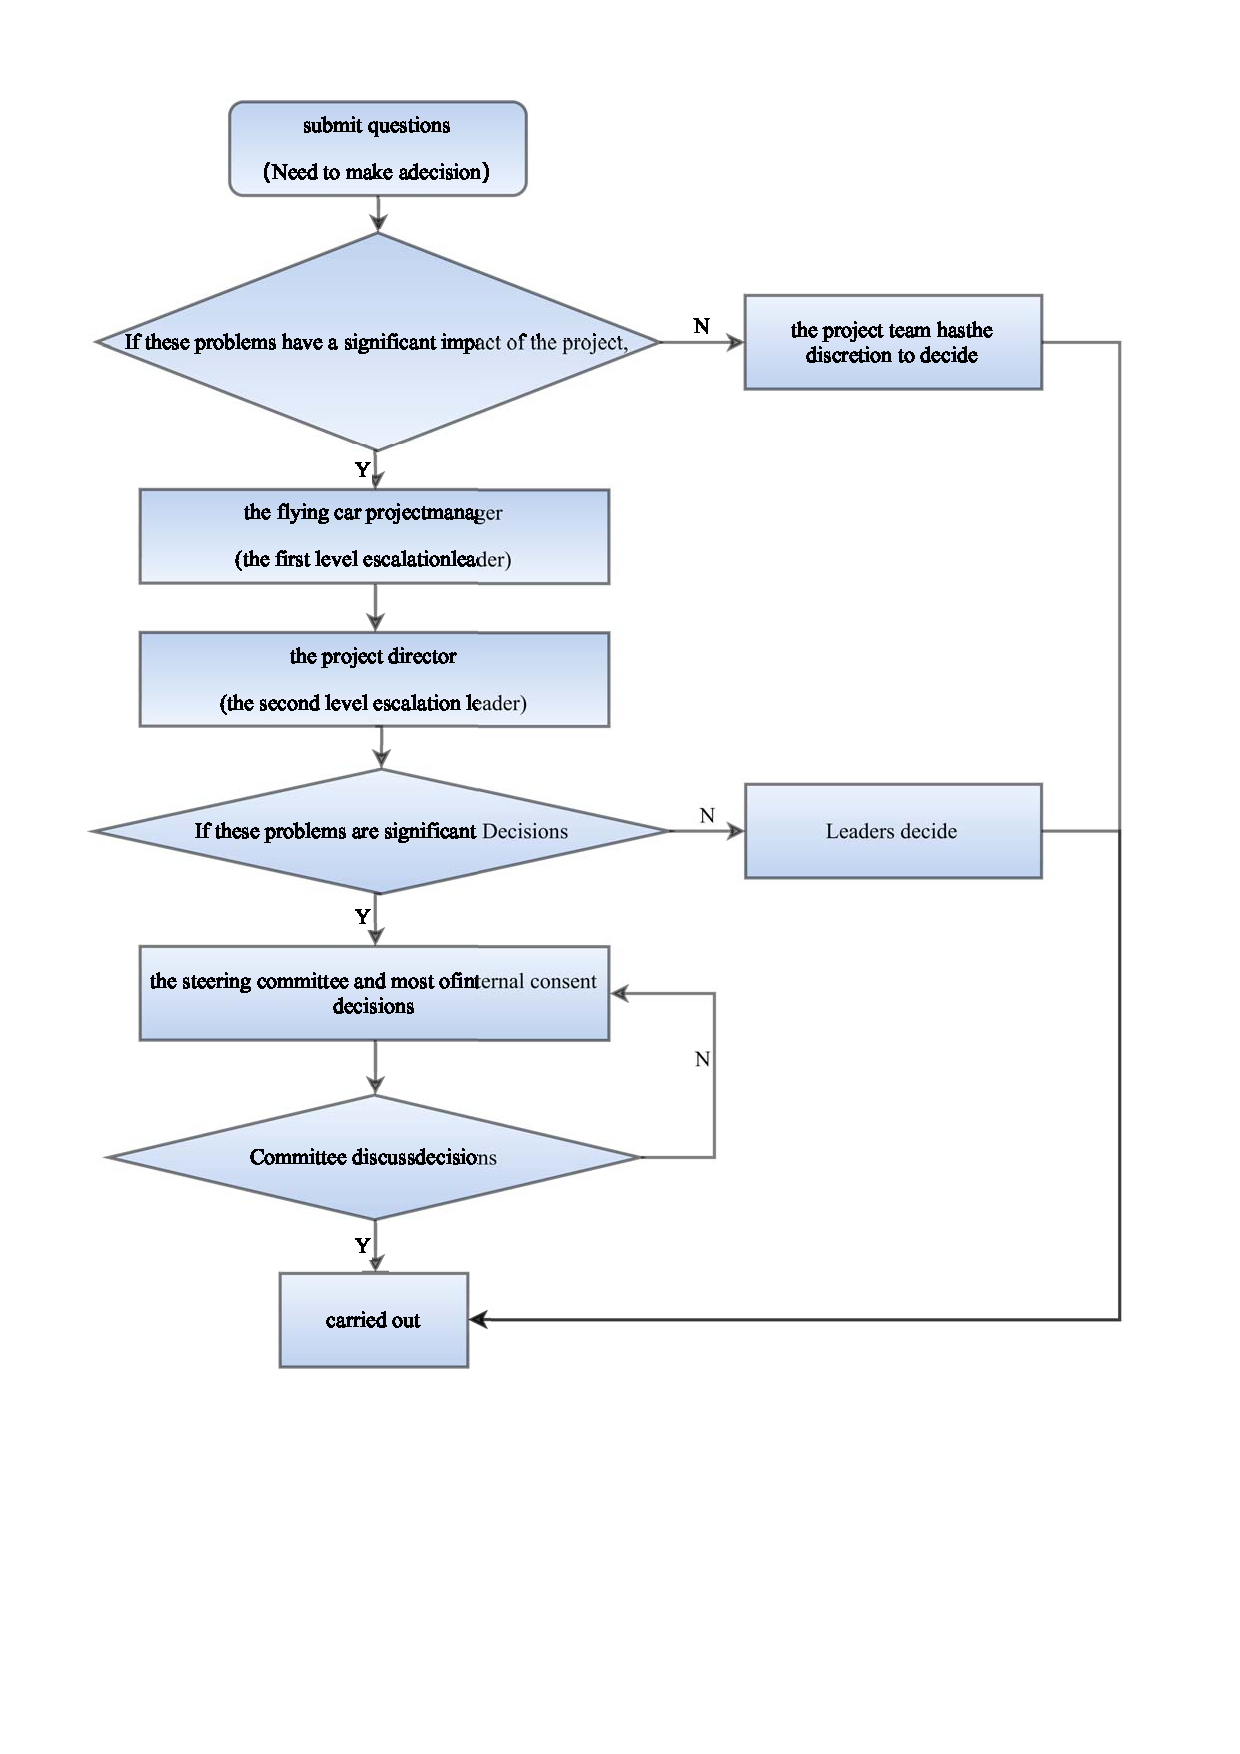
\includegraphics[width=14cm]{pic/ProjectDecisionProcess.pdf}
% \caption{单转换超外差接收机\protect\footnotemark}
% \label{fig:dlr_ads-b_receiver}
\end{figure}

\section{Project meeting}

The Flying Car Project Communication Plan is used to clarify the objectives, scope, processes, and plans for communication for project implementation and training to ensure project leadership, guidance, consultants, and working groups receive timely and accurate information. The target audience for project communication is:

\begin{itemize}
\item Steering Committee
\item Project Director
\item project manager
\item Core project team
\item End user
\end{itemize}

Every Thursday 14:00-15:00 All members of the project team will meet once. The meeting was hosted by the project manager and worked for the past week. To summarize, discuss the problems and solutions in the project work, and arrange the work for next week. Project team and the special project meeting of the management team will arrange the dates according to the situation.

Every Friday 14:00-15:00 The project holds a management meeting, including flying car project director, project manager, and small group leader. At the meeting, the project status report submitted by the project management team will be received, and the project management status report submitted once a week will be taken as develop the main basis for the Steering Committee's report. Project director's development and submission of the steering committee status report and organization of the report work is primarily responsible.



